\documentclass[11pt,letterpaper]{article}

\usepackage[utf8]{inputenc}
\usepackage[spanish,es-nodecimaldot]{babel}
\usepackage{graphicx}

\usepackage{mathtools}
\usepackage{tikz}
\usetikzlibrary{trees,positioning}

\usepackage[top=1in, bottom=1in, left=1in, right=1in]{geometry}


\begin{document}

\begin{titlepage}
    \centering

    {\scshape\LARGE Universidad Nacional Autónoma de México \par}

    \vspace{1cm}
    {\scshape\Large Facultad de Ciencias\par}
    \vspace{1.5cm}

    \begin{center}
        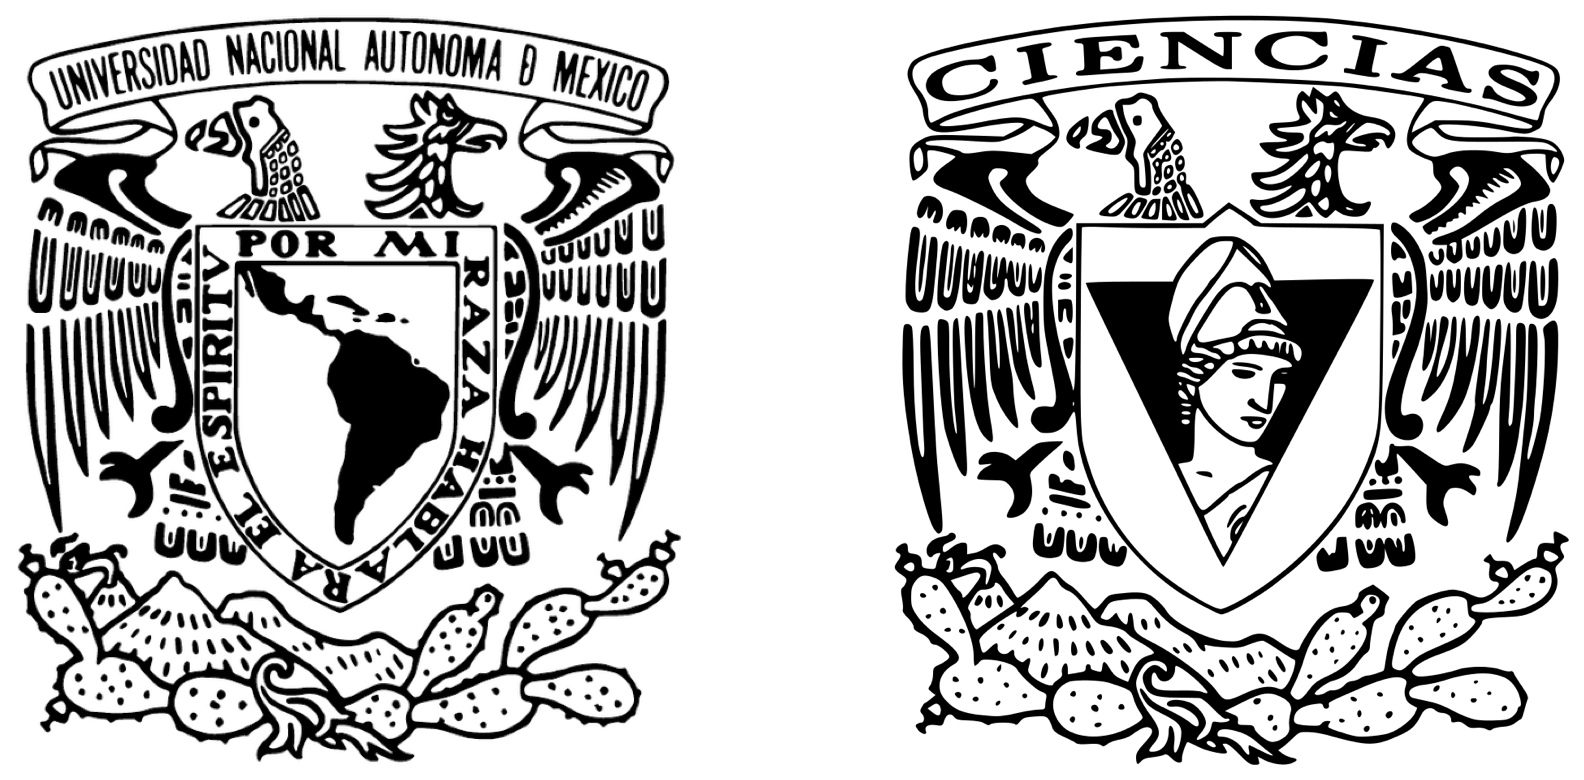
\includegraphics[scale=.1]{../../assets/img/logo.png}
    \end{center}

    \vspace{.8 cm}

    {\LARGE Tarea semanal 02: \par}
    {\huge\bfseries Lógica proposicional \par}

    \vspace{0.5cm}
    {\large\itshape Pablo A. Trinidad Paz\par}
    419004279

    \vfill

    Trabajo presentado como parte del curso de \textbf{Estructuras Discretas}
    impartido por la profesora \textbf{Pilar Selene Linares Arévalo}. \par
    \vspace{0.1cm}
    {\large 29 de agosto de 2018\par}
\end{titlepage}

\begin{enumerate}
    \item Encuentra el valor de verdad para las fórmulas generadas por los
    siguientes árboles de derivación, en el estado de las variables $p = 1$,
    $r = 1$ y $q = 1$.
        \begin{enumerate}
            \item hola \\
                \begin{tikzpicture}[nodes={draw,circle}]
                    \node {E}
                    child {node {F}
                    }
                    child {node {+}
                    }
                    child {node {T}
                    child {node {T}
                      child {node {F}  child {node {8}} }
                      }
                    child {node {*}}
                    child {node {F} child {node {2}}}
                    };
                \end{tikzpicture}
        \end{enumerate}
\end{enumerate}

\end{document}
